R-CNN 其实是一个很大的家族,自从Ross Girshick发表\textit{Rich feature hierarchies for accurate object detection and semantic segmentation}\cite{rcnn},子孙无数、桃李满天下。在此,我们只探讨 R-CNN 直系亲属,他们的发展顺序如下:

\vspace{10pt}
%%%%%%%%%%%%%%%%%%%%%%%%%%%将要提到glossary文档中%%%%%%%%%%%%%%%%%%%%%%%%%%%%%

\begin{tikzpicture}[node distance=3cm]
\node (rcnn) [Node]
{R-CNN};
\node (sppnet) [Node,right of=rcnn]
{SPP-Net};
\node (fastrcnn) [Node,right of=sppnet]
{Fast R-CNN};
\node (fasterrcnn) [Node,right of=fastrcnn]
{Faster R-CNN};
\node (maskrcnn) [Node,right of=fasterrcnn]
{Mask R-CNN};
%连接具体形状
\draw [arrow] (rcnn) -- (sppnet);
\draw [arrow] (sppnet) -- (fastrcnn);
\draw [arrow] (fastrcnn) -- (fasterrcnn);
\draw [arrow] (fasterrcnn) -- (maskrcnn);
\end{tikzpicture}

他们在整个家族进化的过程中,一致暗埋了一条主线:充分榨干 feature maps 的价值。

\subsubsection{R-CNN}
Region CNN(RCNN)\cite{rcnn}可以说是利用深度学习进行目标检测的开山之作。作者Ross Girshick多次在PASCAL VOC的目标检测竞赛中折桂,2010年更带领团队获得终身成就奖,如今供职于Facebook旗下的FAIR。图\ref{rcnn}这个模型,是利用卷积神经网络来做“目标检测”的开山之作,其意义深远不言而喻。
\begin{uscfigure}
	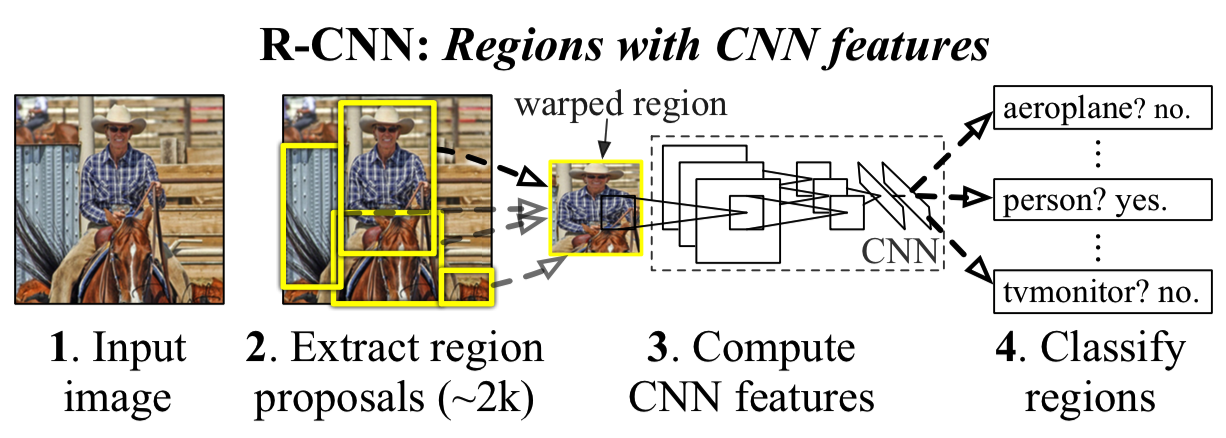
\includegraphics[width=\textwidth]{./Pictures/rcnn-regions_with_cnn_features.png}	
	\caption{RCNN算法框架}
	\label{rcnn}
\end{uscfigure}

本文解决了目标检测中的两个关键问题
\textbf{解决问题一、速度。}
传统的区域选择使用滑窗,每滑一个窗口检测一次,相邻窗口信息重叠高,检测速度慢。R-CNN 使用一个启发式方法(Selective search),先生成候选区域再检测,降低信息冗余程度,从而提高检测速度。

\textbf{解决问题二、训练集。}
经典的目标检测算法在区域中提取人工设定的特征(Haar,HOG)。传统的手工提取特征鲁棒性差,限于如颜色、纹理等 低层次(Low level)的特征。使用CNN(卷积神经网络)提取特征,可以提取更高层面的抽象特征,从而提高特征的鲁棒性。

该方法将PASCAL VOC上的检测率从35.1\% 提升到 53.7 \% ,提高了好几个量级。虽然比传统方法好很多,但是从现在的眼光看,只能是初窥门径。

\textbf{算法流程:}
\begin{itemize}
	\item[>] 一张图像生成1K至2K个候选区域
	\item[>] 对每个候选区域,使用深度网络提取特征
	\item[>] 特征送入每一类的SVM分类器,判别是否属于该类
	\item[>] 使用回归器精细修正候选位置	
\end{itemize}

\textbf{1、候选区域生成:}使用Selective Search方法从一张图像生成约2000-3000个候选区域。基本思路如下:

- 使用一种分割手段,将图像分割成小区域

- 查看现有小区域,合并可能性最高的两个区域。重复直到整张图像合并成一个区域位置

- 输出所有曾经存在过的区域,所谓候选区域

\textbf{2、特征提取:}借鉴Hinton 2012年在Image Net上的分类网络,提取特征。

\textbf{3、类别判断:}对每一类目标,使用一个线性SVM二类分类器进行判别。输入为深度网络输出的4096维特征,输出是否属于此类。 由于负样本很多,使用hard negative mining方法。

\textbf{4、位置精修:}目标检测问题的衡量标准是重叠面积:许多看似准确的检测结果,往往因为候选框不够准确,重叠面积很小。故需要一个位置精修步骤。 

\subsubsection{SPP Net}
R-CNN提出后的一年,以何恺明、任少卿为首的团队发表了\textit{Spatial pyramid pooling in deep convolutional networks for visual recognition}(SPP Net)\cite{sppnet} ,这才是真正摸到了卷积神经网络的脉络。也不奇怪,毕竟这些人鼓捣出了 ResNet 残差网络,对神经网络的理解是其他人没法比的。尽管 R-CNN 效果不错,但是他还有两个硬伤:

\textbf{硬伤一、算力冗余。}
先生成候选区域,再对区域进行卷积,这里有两个问题:其一是候选区域会有一定程度的重叠,对相同区域进行重复卷积;其二是每个区域进行新的卷积需要新的存储空间。何恺明等人意识到这个可以优化,于是把先生成候选区域再卷积,变成了先卷积后生成区域。“简单地”改变顺序,不仅减少存储量而且加快了训练速度。

\textbf{硬伤二、图片缩放。}
无论是剪裁(Crop)还是缩放(Warp),在很大程度上会丢失图片原有的信息导致训练效果不好,如图\ref{sppnet}所示。直观的理解,把车剪裁成一个门,人看到这个门也不好判断整体是一辆车;把一座高塔缩放成一个胖胖的塔,人看到也没很大把握直接下结论。人都做不到,机器的难度就可想而知了。
\begin{uscfigure}
	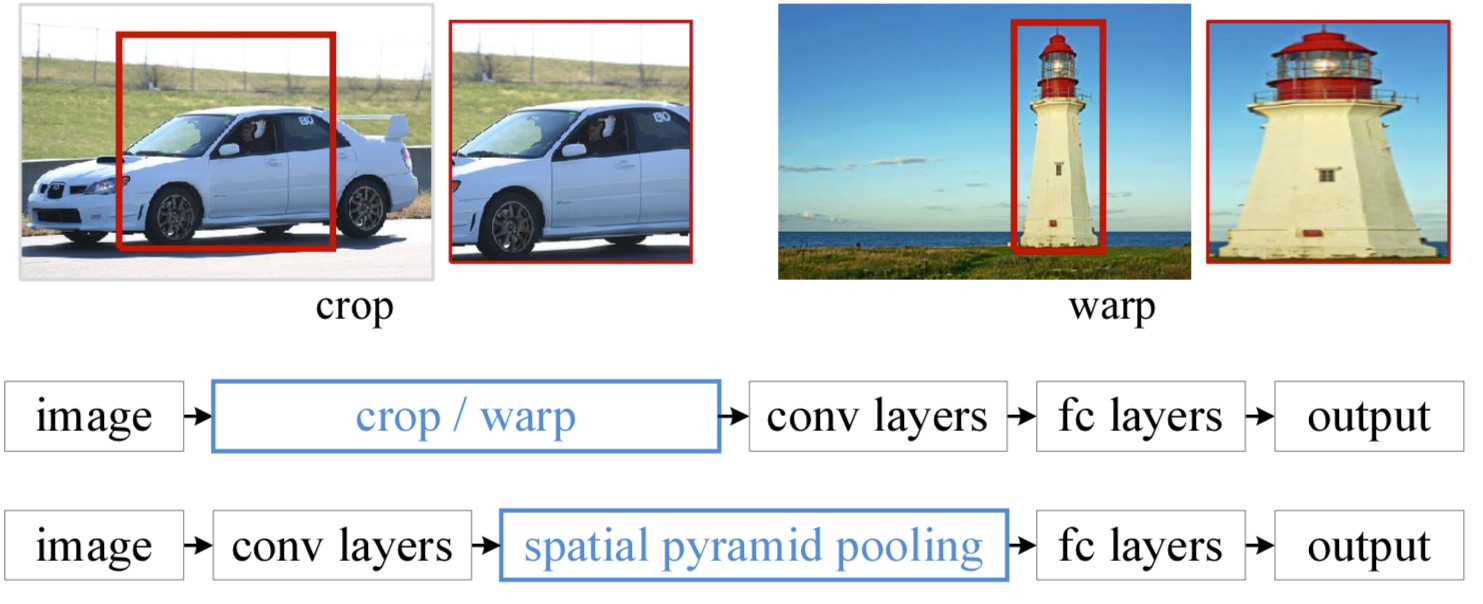
\includegraphics[width=\textwidth]{./Pictures/sppnet_crop_warp.jpg}	
	\caption{因剪裁和绽放导致的信息丢失}
	\label{sppnet}
\end{uscfigure}
何恺明等人发现了这个问题,于是思索有什么办法能不对图片进行变形,将图片原汁原味地输入进去学习。最后,他们发现问题的根源是 FC Layer(全连接层)需要确定输入维度,于是他们在输入全连接层前定义一个特殊的池化层,将输入的任意尺度 feature maps 组合成特定维度的输出,这个组合可以是不同大小的拼凑,如同拼凑七巧板般。举个例子,我们要输入的维度 $64∗256$ ,那么我们可以这样组合 $32∗256+16∗256+8∗256+8∗256$。
\begin{uscfigure}
	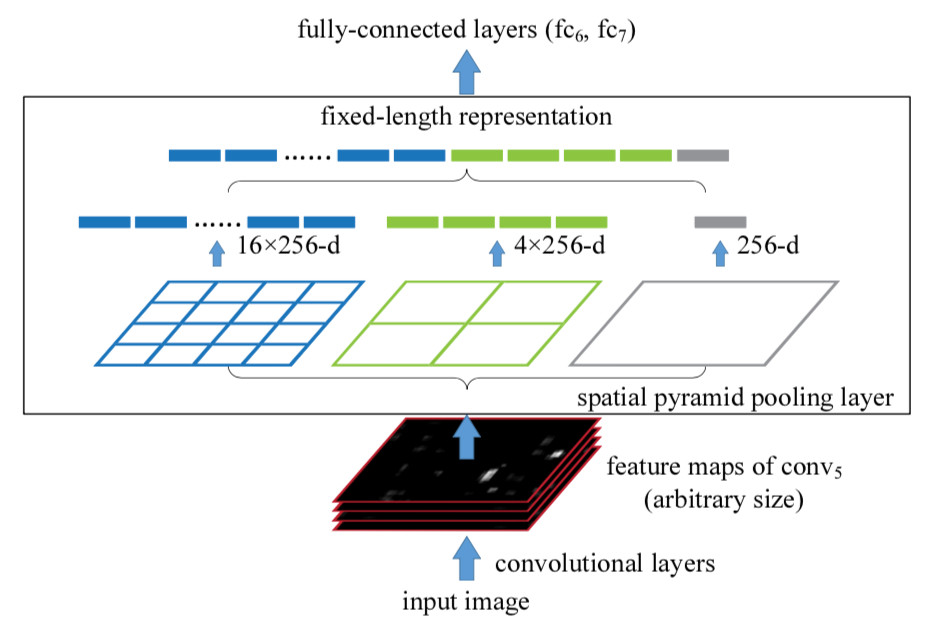
\includegraphics[width=\textwidth,]{./Pictures/sppnet_pool_layer.jpg}	
	\caption{输入维度的组合方式}
\end{uscfigure}
SPP Net 的出现是如同一道惊雷,不仅减少了计算冗余,更重要的是打破了固定尺寸输入这一束缚,让后来者享受到这一缕阳光。

\subsubsection{Fast R-CNN}
继2014年的RCNN之后,Ross Girshick在15年推出Fast RCNN,构思精巧,流程更为紧凑,大幅提升了目标检测的速度。2015年Girshick,Ross发表了\textit{Fast r-cnn}\cite{fastrcnn},在这篇论文中,引用了 SPP Net 的工作,并且致谢其第一作者何恺明的慷慨解答。纵观全文,最大的建树就是将原来的串行结构改成并行结构。同样使用最大规模的网络,Fast RCNN和RCNN相比,训练时间从84小时减少为9.5小时,测试时间从47秒减少为0.32秒。在PASCAL VOC 2007上的准确率相差无几,约在66\%-67\%之间。其算法框架如图\ref{fast-rcnn}
\begin{uscfigure}
	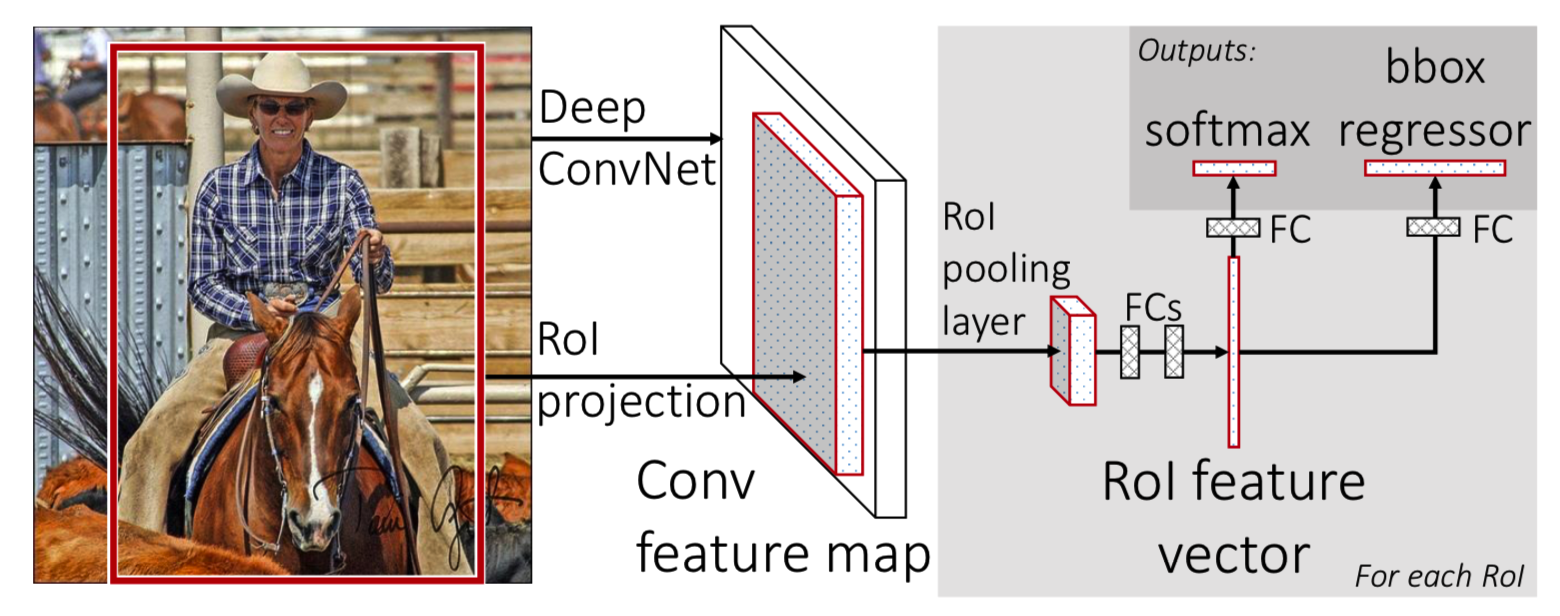
\includegraphics[width=\textwidth]{./Pictures/fast_rcnn.png}	
	\caption{Fast R-CNN算法框架}	
	\label{fast-rcnn}
\end{uscfigure}
原来的R-CNN是先对候选框区域进行分类,判断有没有物体,如果有则对Bounding Box进行精修、回归。这是一个串联式的任务,那么势必没有并联的快,所以Ross Girshick就将原有结构改成并行——在分类的同时,对Bbox进行回归。这一改变将Bbox和Clf的loss结合起来变成一个Loss一起训练,并吸纳了SPP Net的优点,最终不仅加快了预测的速度,而且提高了精度。

简单来说,RCNN使用以下四步来实现目标检测:
\begin{itemize}
	\item[>] 在图像中确定1000-2000个候选框 
	\item[>] 对于每个候选框内图像块,使用深度网络提取特征
	\item[>] 对候选框中提取出的特征,使用分类器判别是否属于一个特定类
	\item[>] 对于属于某一特征的候选框,用回归器进一步调整位置
\end{itemize}
Fast RCNN方法解决了RCNN方法三个问题:

\textbf{问题一、测试时速度慢。}RCNN一张图像内候选框之间大量重叠,提取特征操作冗余,本文将整张图像归一化后直接送入深度网络。在邻接时,才加入候选框信息,在末尾的少数几层处理每个候选框。

\textbf{问题二、训练时速度慢。}原因同问题一,在训练时,本文先将一张图像送入网络,紧接着送入从这幅图像上提取出的候选区域。这些候选区域的前几层特征不需要再重复计算。

\textbf{问题三、训练所需空间大。}RCNN中独立的分类器和加归器需要大量特征作为训练样,本文把类别判断和位置精调统一用深度网络实现,不再需要额外存储。其网络模型如图\ref{fast-rcnn-model}

\begin{uscfigure}
	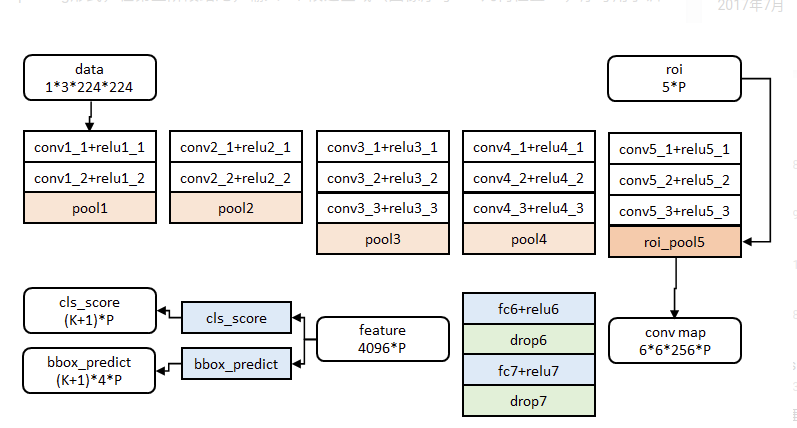
\includegraphics[width=\textwidth]{./Pictures/fast-rcnn-model.png}	
	\caption{Fast R-CNN网络模型}	
	\label{fast-rcnn-model}
\end{uscfigure}

\textbf{损失函数:}
loss\_cls层评估分类代价。由真实分类$u$对应的概率决定:
\[
	L_{cls} = - \log p_u
\]
loss\_bbox评估检测框定位代价。比较真实分类对应的预测参数$t^u$和真实平移绽放为$v$的差别:
\[
	L_{loc} = \sum_{i=1}^{4} g(t_i^u - v_i)
\]
g为Smooth L1误差,对outlier不敏感:
\begin{equation}
	g(x) = \left \{
		\begin{aligned}
		& 0.5x^2 	 & |x| < 1	\\	
		& |x| - 0.5  &otherwise
		\end{aligned}
		\right .
\end{equation}
总代价为两者加权和,如果分类为背景则不考虑定位代价:
\begin{equation}
	L = \left \{
		\begin{aligned}
		& L_{cls} + \lambda L_{loc} & u\\
		& L_{cls} 					& u
		\end{aligned}
	\right .
\end{equation}
\subsubsection{Faster R-CNN}
继RCNN,Fast RCNN之后,目标检测界的领军人物Ross Girshick团队在2015年的又一力作。简单网络目标检测速度达到17fps,在PASCAL VOC上准确率为59.9\%;复杂网络达到5fps,准确率78.8\%。在Faster R-CNN前,我们生产候选区域都是用的一系列启发式算法,基于Low Level特征生成区域。这样就有两个问题:

\textbf{第一个问题}是生成区域的靠谱程度随缘,而“two stage”算法正是依靠生成区域的靠谱程度——生成大量无效区域则会造成算力的浪费、少生成区域则会漏检;

\textbf{第二个问题}是生成候选区域的算法是在CPU上运行的,而我们的训练在GPU上面,跨结构交互必定会有损效率。

那么怎么解决这两个问题呢?于是乎,任少卿等人提出了一个Region Proposal Networks的概念,利用神经网络自己学习去生成候选区域。其结构如图\ref{rpn}。
\begin{uscfigure}
	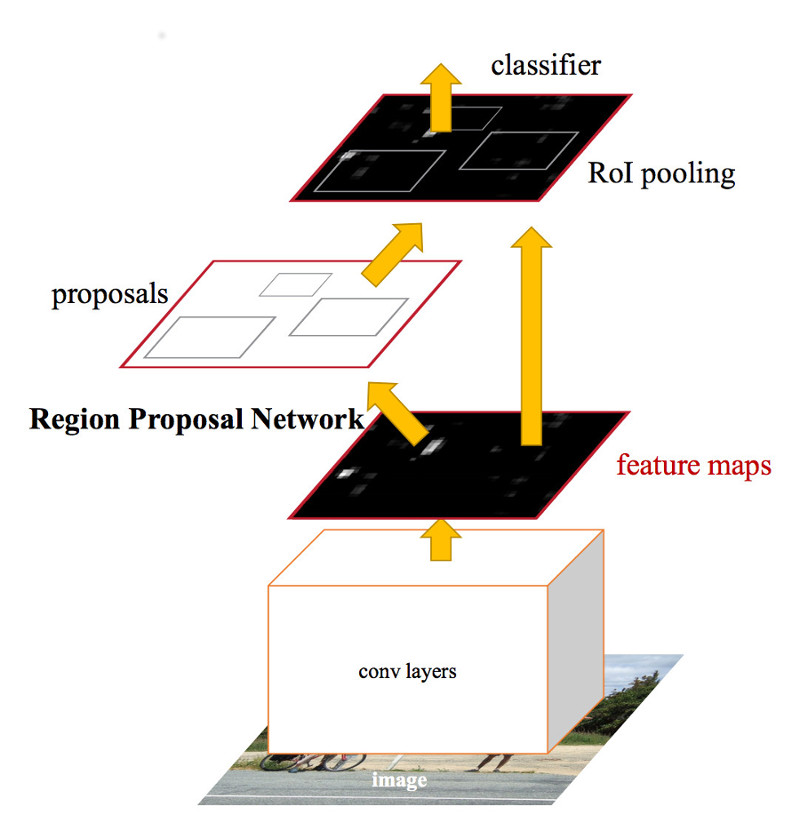
\includegraphics[width=\textwidth,height=8cm]{./Pictures/faster_rcnn.jpg}	
	\caption{RPN结构}	
	\label{rpn}
\end{uscfigure}
这种生成方法同时解决了上述的两个问题,神经网络可以学到更加高层、语义、抽象的特征,生成的候选区域的可靠程度大大提高;可以从上图看出RPNs和RoI Pooling共用前面的卷积神经网络——将RPNs嵌入原有网络,原有网络和RPNs一起预测,大大地减少了参数量和预测时间。在 RPNs 中引入了anchor的概念feature map中每个滑窗位置都会生成k个anchors,然后判断anchor覆盖的图像是前景还是背景,同时回归Bbox的精细位置,预测的Bbox更加精确。

从RCNN到fast RCNN,再到本文的faster RCNN,目标检测的四个基本步骤(候选区域生成,特征提取,分类,位置精修)终于被统一到一个深度网络框架之内。所有计算没有重复,完全在GPU中完成,大大提高了运行速度。

Faster RCNN着重解决了三个问题:
\begin{itemize}
	\item[>] 如何设计区域生成网络
	\item[>] 如何训练区域生成网络
	\item[>] 如何让区域生成网络和Faster RCNN网络共享特征提取网络
\end{itemize}
\textbf{区域生成网络(RPN)}
\begin{uscfigure}
	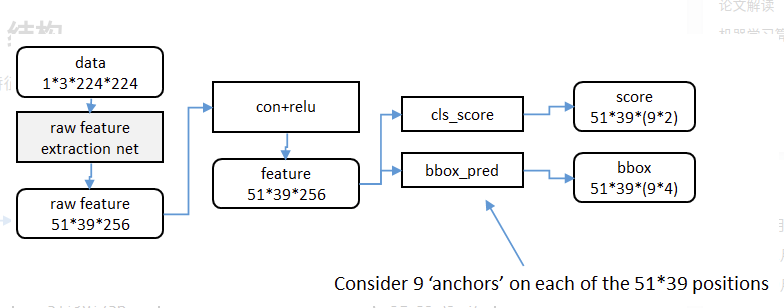
\includegraphics[width=\textwidth,height=8cm]{./Pictures/rpn.png}	
	\caption{RPN结构}	
	\label{rpn-model}
\end{uscfigure}
\subsubsection{Mask R-CNN}
时隔一年,何恺明团队再次更新了 R-CNN 家族,改进 Faster R-CNN 并使用新的 backbone 和 FPN 创造出了 Mask R-CNN 。

\textbf{加一条通道。}我们纵观发展历史,发现SPP Net升级为Fast R-CNN时结合了两个loss,也就是说网络输入了两种信息去训练,结果精度大大提高了。何恺明他们就思考着再加一个信息输入,即图像的Mask,信息变多之后会不会有提升呢?于是乎Mask R-CNN就这样出来了,不仅可以做“目标检测”还可以同时做“语义分割”,将两个计算机视觉基本任务融入一个框架。没有使用什么trick,性能却有了较为明显的提升,这个升级的版本让人们不无啧啧惊叹。作者称其为meta algorithm ,即一个基础的算法,只要需要“目标检测”或者“语义分割”都可以使用这个作为Backbone。


